\documentclass[spanish,12pt,a4paper,titlepage]{report}
\usepackage[utf8]{inputenc}
\usepackage{graphicx}
\usepackage{subfig}
\usepackage{float}
\usepackage{wrapfig}
\usepackage{multirow}
\usepackage{caption}
\usepackage[spanish]{babel}
\usepackage[dvips]{hyperref}
\usepackage{amssymb}
\usepackage{listings}
\usepackage{epsfig}
\usepackage{amsmath}
\usepackage{array}
\usepackage[table]{xcolor}
\usepackage{multirow}
%\usepackage[Sonny]{fncychap}
\usepackage[Lenny]{fncychap}
%\usepackage[Glenn]{fncychap}
%\usepackage[Conny]{fncychap}
%\usepackage[Rejne]{fncychap}
%\usepackage[Bjarne]{fncychap}
%\usepackage[Bjornstrup]{fncychap}

%\usepackage{subfiles}
%\usepackage{framed}

\setlength{\topmargin}{-1.5cm}
\setlength{\textheight}{25cm}
\setlength{\oddsidemargin}{0.3cm} 
\setlength{\textwidth}{15cm}
\setlength{\columnsep}{0cm}


\begin{document}

\chapter{Caracterización de los motores}
\section{Objetivo}
El objetivo de este Test es el de caracterizar el funcionamiento de los motores. Con dicho fin se busca determinar:

\begin{itemize}
\item Relación entre velocidad angular y fuerza
\item Relación entre comando I2C y la velocidad angular.
\item Relación entre comando I2C y la fuerza
\end{itemize}

La primer relación sirve para desprendernos de uno de los parámetros a la hora de realizar el control. Del mismo modo sirve para verificar que la respuesta de los motores verifica las relaciones estudiadas en diversas bibliografías.\\

La segunda es fundamental de conocer ya que lo que el procesador controlará es un comando I2C y no directamente la velocidad del motor. \\

La tercer relación resulta redundante conociendo las anteriores. Sin embargo parece interesante realizar dicho relevamiento a fin de verificar que no surja ninguna inconsistencia. \\
\section{Materiales}
\begin{itemize}
\item Motores
\item LED IR
\item Detector IR
\item Balanza
\item Morsa
\item Beagleboard
\end{itemize}

\section{Procedimiento}

\subsection{Consideraciones previas}
\subsubsection*{Funcionamiento del dispositivo IR}
Es necesario entender el funcionamiento del \emph{detector IR} para poder realizar un experimento adecuado. Dicho dispositivo es sensible a las \emph{radiaciones infrarrojas}. Si se lo expone a una luz infrarroja constante la salida del dispositivo es un ``1" lógico. Del mismo modo, si se quita dicha fuente de luz la salida continúa siendo un ``1''. \\

En la hoja de datos del dispositivo se explica que mientras se recibe una onda cuadrada de frecuencia 56kHz la salida del mismo es un ``0". Por lo tanto para poder distinguir cuando llega la radiación emitida por la LED de cuando no llega se debe hacer que esta última conmute entre ON y OFF con una frecuencia de 56kHz. Dicho de otro modo, el detector IR debe recibir la información modulada en una frecuencia de 56kHz para luego decodificarla.

\subsubsection*{Diseño del circuito de medida de velocidad angular}

La idea del dispositivo de medida es sencilla. Se trata de hacer ``pasar" la radiación infrarroja emitida por el LED a través de la hélice en funcionamiento de uno de los motores. Esta radiación es recogida del otro lado por el receptor IR.\\

De este modo tendremos a la salida del detector, pulsos de frecuencia correspondientes a la velocidad con la que la hélice obstruye el camino entre el sensor y la LED. \textbf{La velocidad angular será entonces la mitad de dicha frecuencia}.\\ 

\begin{wrapfigure}{l}{0.55\textwidth}
  \vspace{-20pt}
  \begin{center}
    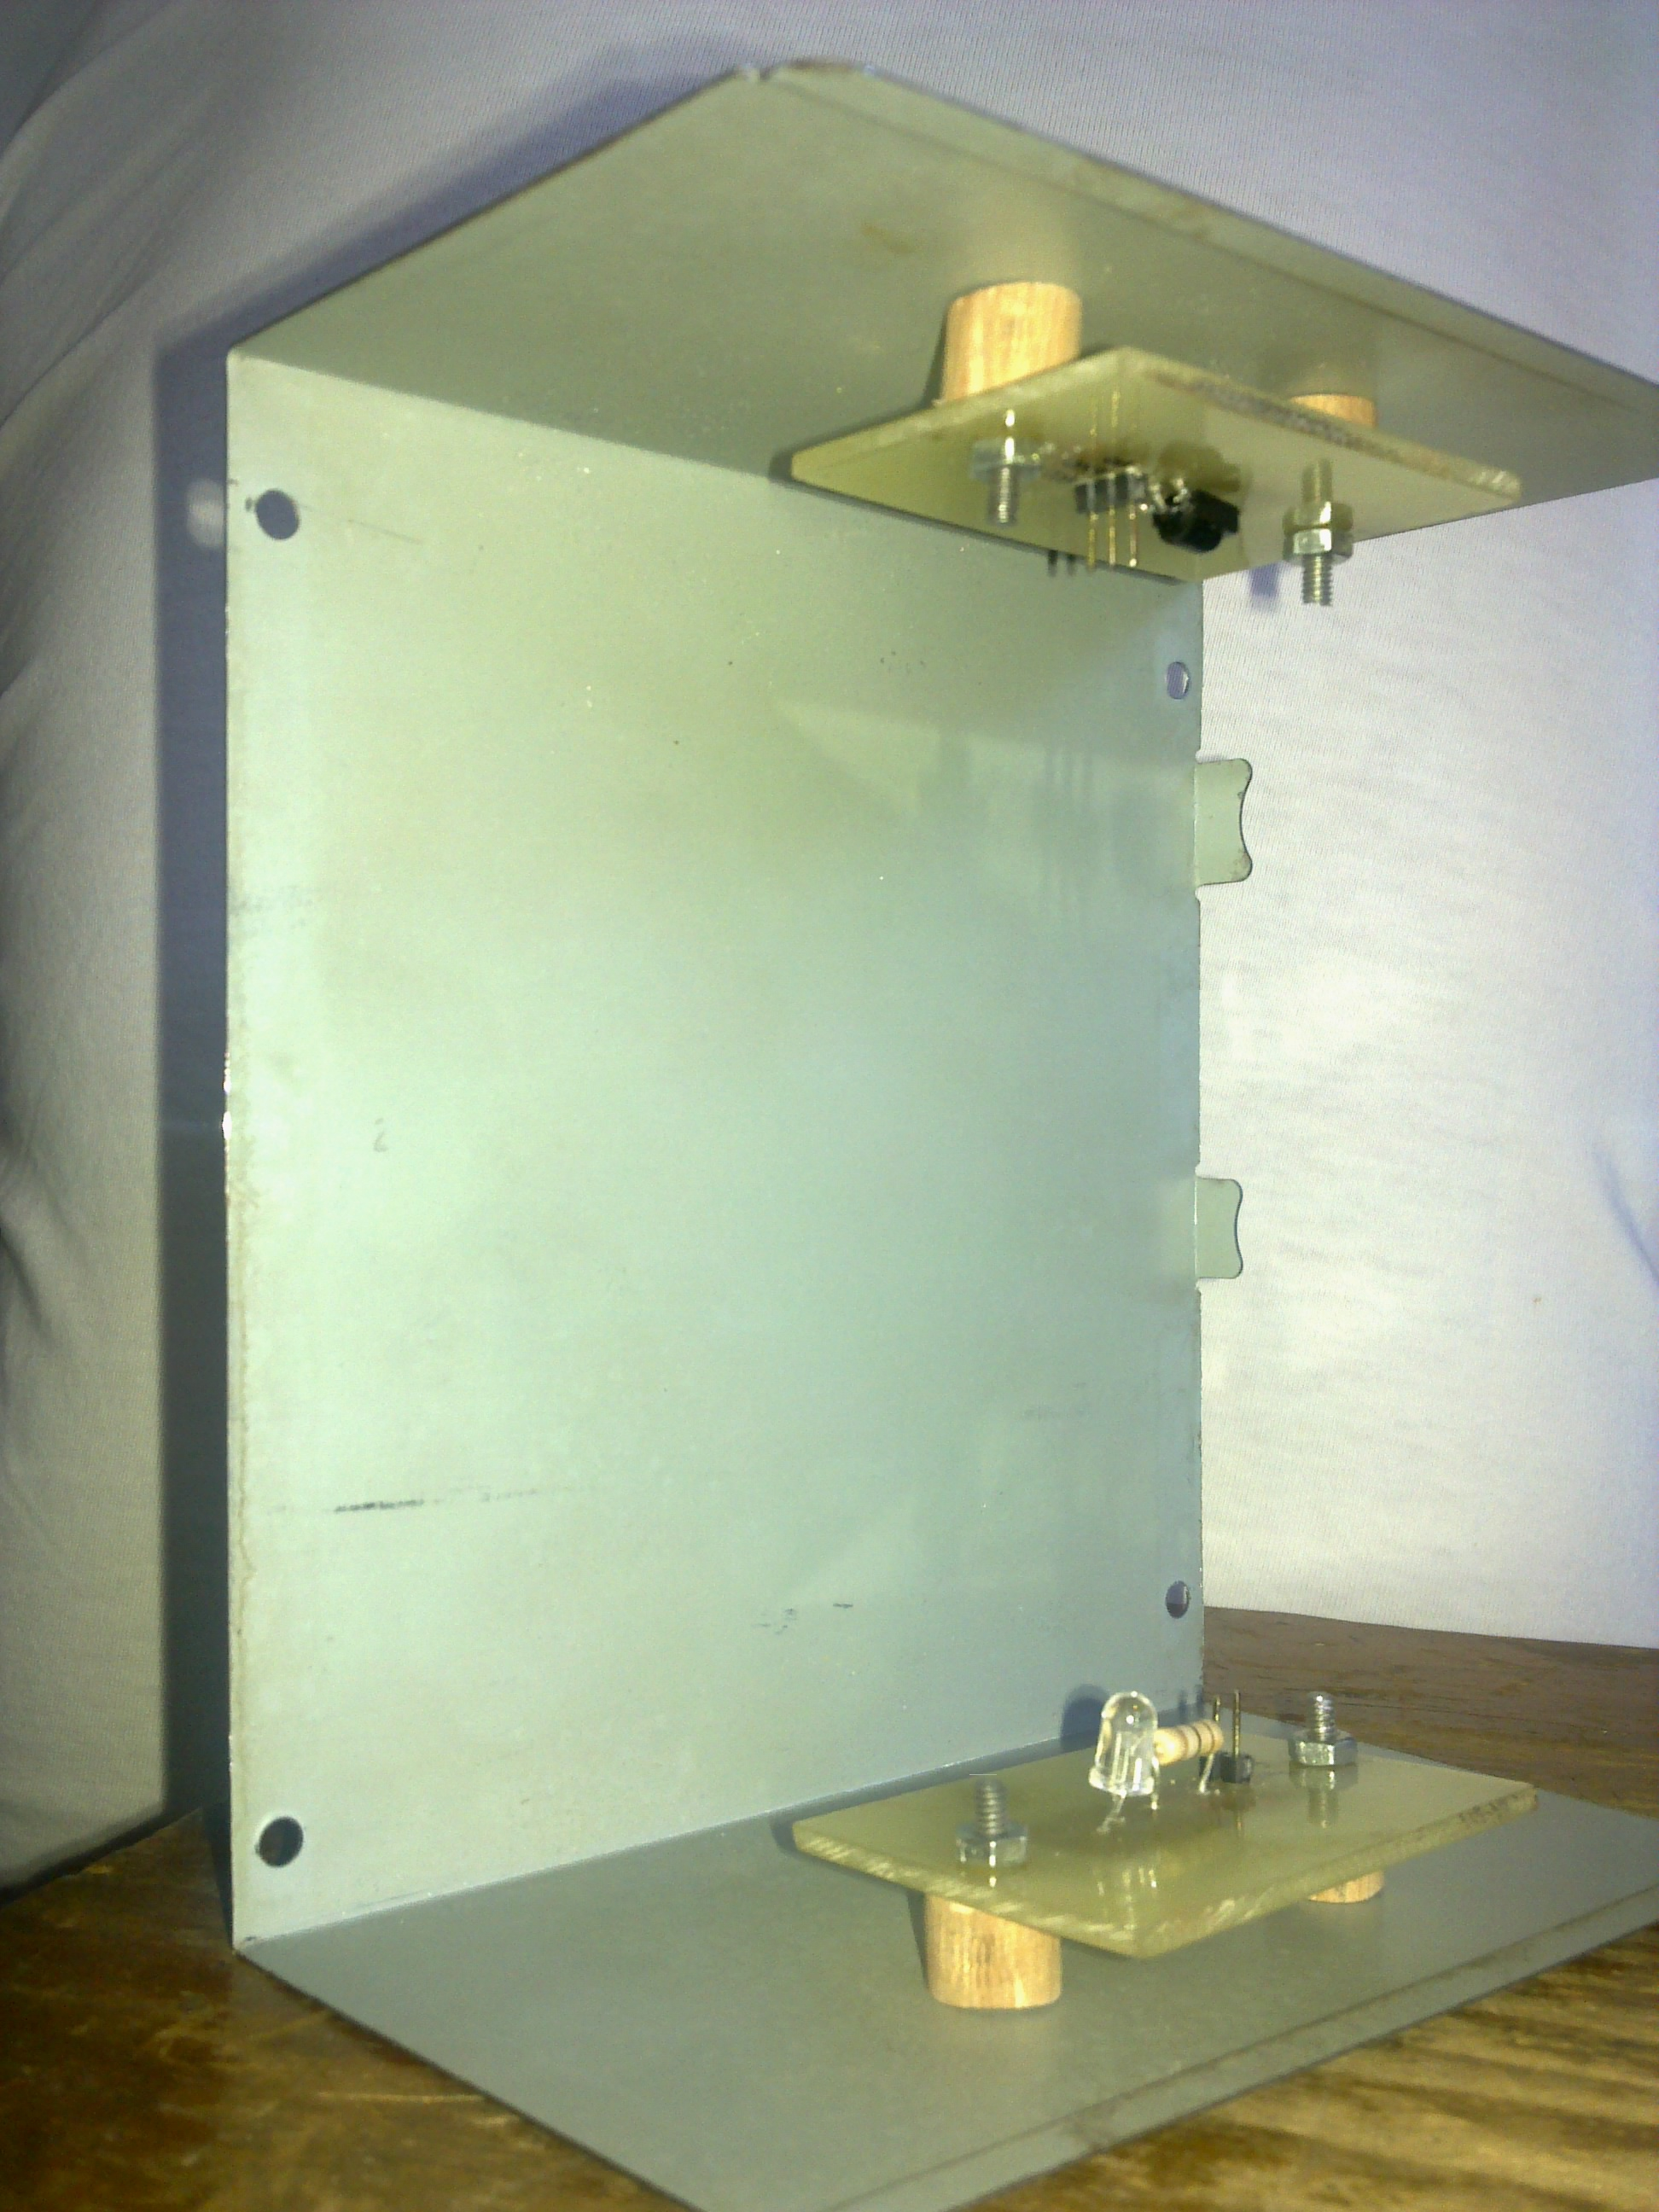
\includegraphics[width=0.42\textwidth]{./Pics/u.jpg}
  \end{center}
  \vspace{-20pt}
  \caption{Dispositivo en forma de U}
  \label{fig:u}
  \vspace{-10pt}
\end{wrapfigure}

El dispositivo se trata de un cuerpo en forma de ``U", donde de un lado se tiene la LED infrarroja y del otro el detector, tal como se puede ver en la figura \ref{fig:u}.\\

Como explicamos anteriormente la LED debe ser conmutada con una frecuencia de 56kHz por lo tanto se la alimentará con un generador de señales funcionando como generador de onda cuadrada a dicha frecuencia. Para lograr un correcto funcionamiento de la misma se requiere una corriente superior a los $100mA$. La amplitud de la onda cuadrada se regulará a $5V$ y se trabajará con una resistencia de $20\Omega$ en serie. Midiendo la tensión en la resistencia se puede comprobar que dichos valores son adecuados para el propósito.\\

La salida del receptor IR se conecta directamente a un frecuencímetro.\\

\subsection{Tests a realizar}

\subsubsection*{Obtención de la curva fuerza contra velocidad angular}

Se sujeta el motor gracias a una morsa y se coloca sobre la balanza. A priori la morsa es suficientemente pesada como para que el empuje del motor no supere el peso de la misma. Moviendo las palancas del control remoto se le imprime mayor velocidad a las hélices lo cual producirá un aumento del empuje. Dicha variación se refleja en la disminución de la lectura de la balanza. 
Simultáneamente, gracias al dispositivo IR, se medirá la velocidad angular con la cual gira el motor. 

Se tomarán medidas para distintas posiciones de la palanca.

\subsubsection*{Obtención de la curva valor del comando I2C contra velocidad angular y de la curva valor del comando I2C contra fuerza}

Luego de estudiados los comandos que se utiliza para comandar los motores y una vez que la BeagleBoard se encuentra capacitada para comunicarse a través de un protocolo I2C se puede proceder a desarrollar esta prueba. En la misma configuración que en los experimentos anteriores se procede a medir los valores de velocidad angular y empuje producidos por los motores. 

Se tomaran medidas para todos los valores posibles del comando I2C, es decir entre 0 y 255.

\section{Resultados y análisis}

\subsubsection{Obtención de la curva fuerza contra velocidad angular}

Luego de apoyar el motor y su soporte sobre la balanza se oprime el botón ``tare". Por lo tanto el peso medido corresponde al opuesto de la fuerza realizada por los motores dividido la constante gravitacional de la Tierra ($9.81ms^{-2}$). Los resultados obtenidos se presentan la tabla \ref{tab:fuerza-vel}.

\begin{table}[H]
\centering
\begin{tabular}{p{80pt}|p{80pt}} 
 \cellcolor[gray]{0.8} \textbf{Peso (g)} & \cellcolor[gray]{0.8} \textbf{Frecuencia (Hz)} \\ \hline
 
 0  & 0  \\ \hline
\cline{1-2}
37 & 34.2\\ \hline
\cline{1-2}
 40  & 35.4  \\ \hline
\cline{1-2}
62 & 43.1\\ \hline
\cline{1-2}
 68  & 44.7  \\ \hline
\cline{1-2}
72 & 47.1\\ \hline
\cline{1-2}
 74  & 47.3  \\ \hline
\cline{1-2}
77 & 49.4\\ \hline
\cline{1-2}
 80  & 49.4  \\ \hline
\cline{1-2}
84 & 50.5\\ \hline
\cline{1-2}
 100  & 54.8  \\ \hline
\cline{1-2}
105 & 56.4\\ \hline
\cline{1-2}
 122  & 60.5  \\ \hline
\cline{1-2}
132 & 62.8\\ \hline
\cline{1-2}
 163  & 70.0  \\ \hline
\cline{1-2}
194 & 75.4\\ \hline
\cline{1-2}
 220  & 80.6  \\ \hline
\cline{1-2}
245 & 83.7\\ \hline
\cline{1-2}
 260  & 86.3  \\ \hline
\cline{1-2}
280 & 90.0\\ \hline
\cline{1-2}
 295  & 91.2  \\ \hline
\cline{1-2}
315 & 95.4\\ \hline
\cline{1-2}
 332  & 37.2  \\ \hline
\cline{1-2}
342 & 98.3\\ \hline
\cline{1-2}
355 & 100.6\\ \hline
\cline{1-2}
360  & 101.0  \\ \hline
\cline{1-2}
420 & 110.0\\ \hline
\cline{1-2}
 440  & 111.9  \\ \hline
\cline{1-2}
444 & 110.5\\ \hline
\cline{1-2}
\end{tabular}
\caption{Medidas obtenidas de peso y frecuencia medida por el dispositivo IR}
\label{tab:fuerza-vel}
\end{table}

Del mismo modo se representa la curva Fuerza-Velocidad angular en la figura \ref{fig:grafica1}.


\begin{figure}
  \vspace{-20pt}
  \begin{center}
    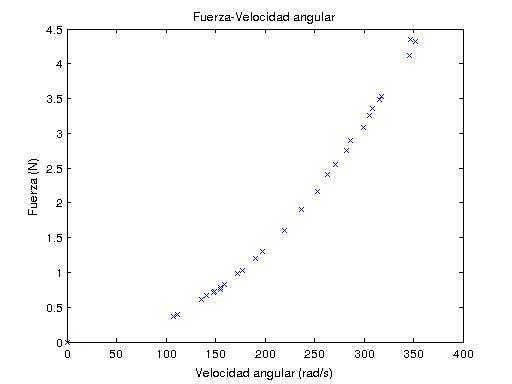
\includegraphics[width=0.8\textwidth]{./Pics/puntosfvel.jpg}
  \end{center}
  \vspace{-20pt}
  \caption{Curva experimental de Fuerza-Velocidad angular}
  \label{fig:grafica1}
  \vspace{-10pt}
\end{figure}


De la observación de los puntos obtenidos se infiere que la respuesta Fuerza-velocidad angular es del tipo cuadrática o cúbica. Suponiendo ambos modelos se obtienen los coeficientes de los polinomios en ambos casos. A partir de dichos coeficientes se grafican las curvas teóricas en ambos casos a fin de compararlas con los puntos obtenidos experimentalmente. Del mismo modo se calcula el error cuadrático medio para ambos modelos propuestos. Los resultados obtenidos se presentan en la figura \ref{fig:grafica2}.


\begin{figure}
  \vspace{-20pt}
  \begin{center}
    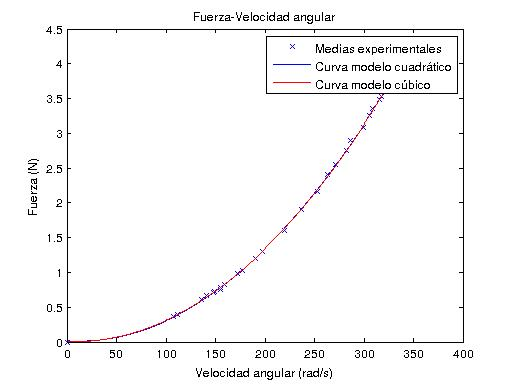
\includegraphics[width=0.8\textwidth]{./Pics/modsfvel.jpg}
  \end{center}
  \vspace{-20pt}
  \caption{Curva de los modelos propuestos para la respuesta Fuerza-Velocidad angular}
  \label{fig:grafica2}
  \vspace{-10pt}
\end{figure}

Como se puede observar en la figura \ref{fig:grafica2} ambas curvas coinciden notablemente entre sí y con los datos experimentales. Por lo tanto podemos afirmar que cualquiera de los dos modelos es adecuado para representar la respuesta Fuerza-velocidad angular. Del mismo modo el error cuadrático medio entre los resultados obtenidos experimentalmente y los resultados predichos por cada modelo es, en ambos casos, 5.4743. Dicha constatación nos permite afirmar que trabajar con el modelo cúbico no nos aporta ninguna ventaja significativa. La razón de esta pequeña diferencia es que el coeficiente que multiplica al término $\omega^3$ es cinco órdenes de magnitud inferior que el coeficiente que multiplica al término $\omega^2$, logrando que el modelo cúbico termine pareciéndose, en definitiva, a un modelo cuadrático.\\

Con los parámetros obtenidos y asumiendo un modelo cuadrático podemos afirmar que la respuesta de los motores Fuerza-Velocidad angular tiene la forma de:

\begin{equation}
3,7646 \times 10^{-5}\omega ^2 - 9,0535 \times 10^{-4}\omega +0.0170
\end{equation}

Donde las unidades del primer coeficiente son $Ns^2$, las del segundo son $Ns$ y las del término independiente son $N$.

Este modelo resulta, además, coherente con la ecuación para el empuje de una hélice:

\begin{equation}
L=\frac{1}{2}\rho V^2S_{ref}C_L
\end{equation}

donde $L$ es la fuerza de elevación (en $N$), $\rho$ es la densidad del aire (en $kg/m^3$), $V$ es la velocidad de giro (en $m/s^2$), $S_{ref}$ es el área de referencia (en $m^2$) (para  una  hélice,  el  área  de  referencia  es  aquella  formada  cuando ésta gira creando un círculo con un radio de la longitud de la hélice) y $C_L$ es el coeficiente de elevación (adimensionado), el cual depende de geometría de la hélice y el ángulo de ataque, entre otros factores.

\end{document}


